\documentclass{article}
\usepackage{enumerate}
\usepackage{amsmath}
\usepackage{amssymb}
\usepackage{graphicx}
\usepackage{subfigure}
\usepackage{geometry}
\usepackage{caption}
\usepackage{indentfirst}
\usepackage{tikz}
\usetikzlibrary{circuits.logic.US}
\usetikzlibrary{arrows.meta}
\usetikzlibrary{calc}
\geometry{left=3.0cm,right=3.0cm,top=3.0cm,bottom=3.0cm}
\renewcommand{\thesection}{Problem \arabic{section}.}
\title{VE270 Homework 8}
\author{Liu Yihao 515370910207}
\date{}

\begin{document}
\maketitle

\section{}
\begin{enumerate}
\item
The truth table is 

\begin{center}
\begin{tabular}{cccc|cccc}
$s_{2}$ & $s_{1}$ & $s_{0}$ & $X$ & $n_{2}$ & $n_{1}$ & $n_{0}$ & $Y$ \\
\hline
0 & 0 & 0 & 0 & 0 & 0 & 0 & 0 \\
0 & 0 & 0 & 1 & 0 & 0 & 1 & 0 \\
0 & 0 & 1 & 0 & 0 & 1 & 1 & 0 \\
0 & 0 & 1 & 1 & 0 & 1 & 0 & 0 \\
0 & 1 & 0 & 0 & 1 & 1 & 0 & 1 \\
0 & 1 & 0 & 1 & 0 & 1 & 0 & 1 \\
0 & 1 & 1 & 0 & 0 & 0 & 0 & 0 \\
0 & 1 & 1 & 1 & 0 & 1 & 0 & 0 \\
1 & 0 & 0 & 0 & X & X & X & X \\
1 & 0 & 0 & 1 & X & X & X & X \\
1 & 0 & 1 & 0 & X & X & X & X \\
1 & 0 & 1 & 1 & X & X & X & X \\
1 & 1 & 0 & 0 & 0 & 0 & 0 & 0 \\
1 & 1 & 0 & 1 & 0 & 1 & 0 & 0 \\
1 & 1 & 1 & 0 & X & X & X & X \\
1 & 1 & 1 & 1 & X & X & X & X \\
\end{tabular}
\end{center}

The euqations are 

$$n_{2}=s_{2}'s_{1}s_{0}'X'$$
$$n_{1}=s_{2}'s_{1}s_{0}'+s_{1}'s_{0}+s_{1}X$$
$$n_{0}=s_{1}'s_{0}'X+s_{1}'s_{0}X'$$
$$Y=s_{2}'s_{1}s_{0}'$$



\item \ 
\begin{center}
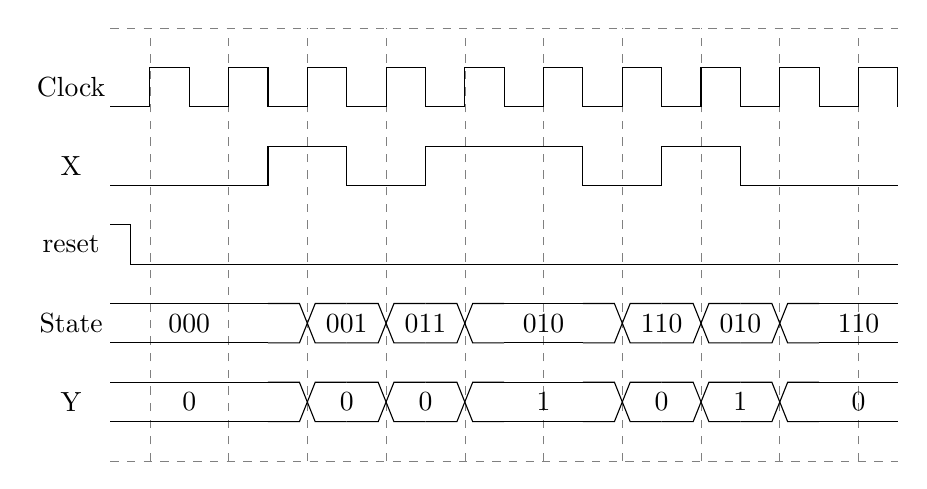
\begin{tikzpicture}
\draw [help lines,dashed] (-0.5,0) grid[xstep=1,ystep=5.5] (9.5,5.5);
\foreach \i in {0,...,9} {
	\draw (\i-0.5,4.5) -- (\i,4.5) -- (\i,5) -- (\i+0.5,5) -- (\i+0.5,4.5);
}
\draw plot[const plot] coordinates {(-0.5,3.5) (1.5,4) (2.5,3.5) (3.5,4) (5.5,3.5) (6.5,4) (7.5,3.5) (9.5,3.5)};
\draw plot[const plot] coordinates {(-0.5,3) (-0.25,2.5) (9.5,2.5)};
\foreach \j in {1,2} {
	\foreach \i in {2,3,4,6,7,8} {
		\draw (\i-0.5,\j) -- (\i-0.1,\j) -- (\i+0.1,\j-0.5) -- (\i+0.5,\j-0.5);
		\draw (\i-0.5,\j-0.5) -- (\i-0.1,\j-0.5) -- (\i+0.1,\j) -- (\i+0.5,\j);
	}
	\foreach \i in {0,1,5,9} {
		\draw (\i-0.5,\j) -- (\i+0.5,\j);
		\draw (\i-0.5,\j-0.5) -- (\i+0.5,\j-0.5);
	}
}
\draw (0.5,1.75) node {000} (2.5,1.75) node {001} (3.5,1.75) node {011} (5,1.75) node {010} (6.5,1.75) node {110} (7.5,1.75) node {010} (9,1.75) node {110};
\draw (0.5,0.75) node {0} (2.5,0.75) node {0} (3.5,0.75) node {0} (5,0.75) node {1} (6.5,0.75) node {0} (7.5,0.75) node {1} (9,0.75) node {0};
\draw (-1,4.75) node {Clock} (-1,3.75) node {X} (-1,2.75) node {reset} (-1,1.75) node {State} (-1,0.75) node {Y};
\end{tikzpicture}
\end{center}

\item
The state diagram is

\begin{center}
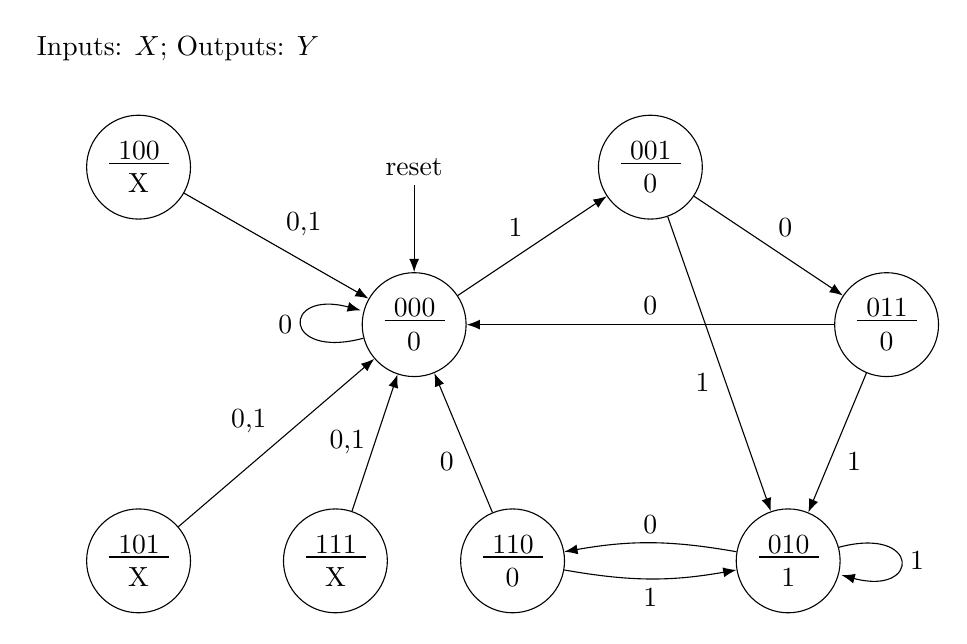
\begin{tikzpicture}[>/.tip={Latex}]
	\draw (-6,2) node (io) {Inputs: $X$; Outputs: $Y$};
	
	\draw (-3,-1.5) node (A) [draw,shape=circle,minimum size=1.25cm,text width=0.75cm,align=center] {\underline{ 000 } 0};
	\draw (0,0.5) node (B) [draw,shape=circle,minimum size=1.25cm,text width=0.75cm,align=center] {\underline{ 001 } 0};
	\draw (3,-1.5) node (C) [draw,shape=circle,minimum size=1.25cm,text width=0.75cm,align=center] {\underline{ 011 } 0};
	\draw (1.75,-4.5) node (D) [draw,shape=circle,minimum size=1.25cm,text width=0.75cm,align=center] {\underline{ 010 } 1};
	\draw (-1.75,-4.5) node (E) [draw,shape=circle,minimum size=1.25cm,text width=0.75cm,align=center] {\underline{ 110 } 0};
	
	\draw (-6.5,0.5) node (F) [draw,shape=circle,minimum size=1.25cm,text width=0.75cm,align=center] {\underline{ 100 } X};
	\draw (-6.5,-4.5) node (G) [draw,shape=circle,minimum size=1.25cm,text width=0.75cm,align=center] {\underline{ 101 } X};
	\draw (-4,-4.5) node (H) [draw,shape=circle,minimum size=1.25cm,text width=0.75cm,align=center] {\underline{ 111 } X};

	\draw[->] (A) edge [loop left] node {0} ();
	\draw[->] (A) edge node [above left] {1} (B);
	\draw[->] (B) edge node [above right] {0} (C);
	\draw[->] (B) edge node [below left] {1} (D);
	\draw[->] (C) edge node [above] {0} (A);
	\draw[->] (C) edge node [below right] {1} (D);
	\draw[->] (D) edge [bend right=10] node [above] {0} (E);
	\draw[->] (D) edge [loop right] node {1} ();
	\draw[->] (E) edge node [below left] {0} (A);
	\draw[->] (E) edge [bend right=10] node [below] {1} (D);
	
	\draw[->] (F) edge node [above right] {0,1} (A);
	\draw[->] (G) edge node [above left] {0,1} (A);
	\draw[->] (H) edge node [left] {0,1} (A);
	
	\draw (-3,0.5) node (reset) {reset};
	\draw[->] (reset) edge (A);
\end{tikzpicture}
\end{center}

The truth table is 

\begin{center}
\begin{tabular}{cccc|cccc}
$s_{2}$ & $s_{1}$ & $s_{0}$ & $X$ & $n_{2}$ & $n_{1}$ & $n_{0}$ & $Y$ \\
\hline
0 & 0 & 0 & 0 & 0 & 0 & 0 & 0 \\
0 & 0 & 0 & 1 & 0 & 0 & 1 & 0 \\
0 & 0 & 1 & 0 & 0 & 1 & 1 & 0 \\
0 & 0 & 1 & 1 & 0 & 1 & 0 & 0 \\
0 & 1 & 0 & 0 & 1 & 1 & 0 & 1 \\
0 & 1 & 0 & 1 & 0 & 1 & 0 & 1 \\
0 & 1 & 1 & 0 & 0 & 0 & 0 & 0 \\
0 & 1 & 1 & 1 & 0 & 1 & 0 & 0 \\
1 & 0 & 0 & 0 & 0 & 0 & 0 & 0 \\
1 & 0 & 0 & 1 & 0 & 0 & 0 & 0 \\
1 & 0 & 1 & 0 & 0 & 0 & 0 & 0 \\
1 & 0 & 1 & 1 & 0 & 0 & 0 & 0 \\
1 & 1 & 0 & 0 & 0 & 0 & 0 & 0 \\
1 & 1 & 0 & 1 & 0 & 1 & 0 & 0 \\
1 & 1 & 1 & 0 & 0 & 0 & 0 & 0 \\
1 & 1 & 1 & 1 & 0 & 0 & 0 & 0 \\
\end{tabular}
\end{center}

The euqations are 

$$n_{2}=s_{2}'s_{1}s_{0}'X'$$
$$n_{1}=s_{2}'s_{1}'s_{0}+s_{2}'s_{0}X+s_{2}'s_{1}s_{0}'+s_{1}s_{0}'X$$
$$n_{0}=s_{2}'s_{1}'s_{0}'X+s_{2}'s_{1}'s_{0}X'$$
$$Y=s_{2}'s_{1}s_{0}'$$


The schematics is 

\begin{center}
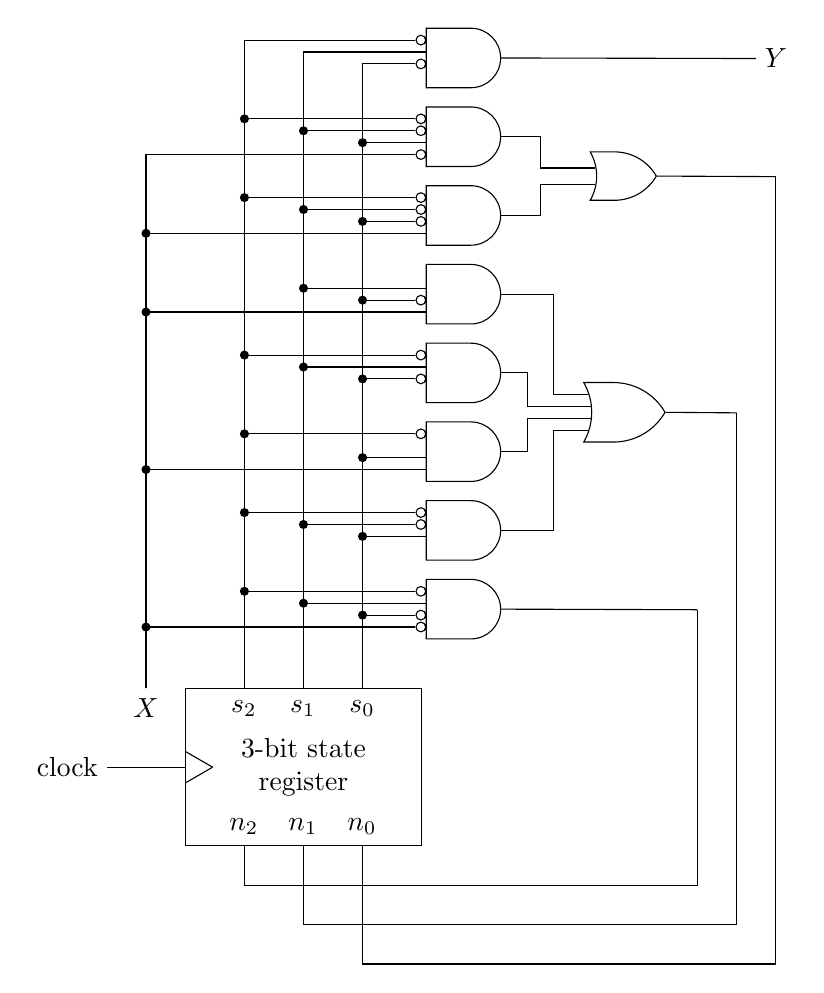
\begin{tikzpicture}[circuit logic US]
\draw (0,0) node (r) [shape=rectangle,draw,minimum height=2cm,minimum width=3cm,text width=2cm,align=center] {3-bit state register};
\draw (-3,0) node (clock) {clock};\draw (clock) -- (r.west);\draw (r) ++(left:11.54mm) -- ++($(left:3.46mm)+(down:2mm)$);
\draw (r) ++(left:11.54mm) -- ++($(left:3.46mm)+(up:2mm)$);
\draw (r.west) ++(up:7.5mm) ++(right:7.500000mm) node {$s_2$};
\draw (r.west) ++(down:7.5mm) ++(right:7.500000mm) node {$n_2$};
\draw (r.west) ++(up:7.5mm) ++(right:15.000000mm) node {$s_1$};
\draw (r.west) ++(down:7.5mm) ++(right:15.000000mm) node {$n_1$};
\draw (r.west) ++(up:7.5mm) ++(right:22.500000mm) node {$s_0$};
\draw (r.west) ++(down:7.5mm) ++(right:22.500000mm) node {$n_0$};
\draw (-2.000000,0.750000) node {$X$};
\draw (r.north) ++(up:1.000000cm) ++(right:2cm) node (and1) [and gate,inputs=inii] {};
\draw (-0.750000,1.000000) |- (and1.input 1) ;
\draw (0.000000,1.000000) |- (and1.input 2) ;
\draw (0.750000,1.000000) |- (and1.input 3) ;
\draw (-2.000000,1.000000) |- (and1.input 4) ;
\draw (and1.output) -- (5.000000,2.000000);
\draw (5.000000,2.000000) -- (5.000000,-1.500000) -| (-0.750000,-1);
\draw (r.north) ++(up:2.000000cm) ++(right:2cm) node (and2) [and gate,inputs=iinn] {};
\draw (-0.750000,1.000000) |- (and2.input 1) ;
\draw (0.000000,1.000000) |- (and2.input 2) ;
\draw (0.750000,1.000000) |- (and2.input 3) ;
\draw (and1.input 1) ;
\pgfgetlastxy{\x}{\y};
\filldraw (-0.750000,\y) circle [radius=0.5mm];
\draw (and1.input 2) ;
\pgfgetlastxy{\x}{\y};
\filldraw (0.000000,\y) circle [radius=0.5mm];
\draw (and1.input 3) ;
\pgfgetlastxy{\x}{\y};
\filldraw (0.750000,\y) circle [radius=0.5mm];
\draw (r.north) ++(up:3.000000cm) ++(right:2cm) node (and3) [and gate,inputs=innn] {};
\draw (-0.750000,1.000000) |- (and3.input 1) ;
\draw (0.750000,1.000000) |- (and3.input 3) ;
\draw (-2.000000,1.000000) |- (and3.input 4) ;
\draw (and2.input 1) ;
\pgfgetlastxy{\x}{\y};
\filldraw (-0.750000,\y) circle [radius=0.5mm];
\draw (and2.input 3) ;
\pgfgetlastxy{\x}{\y};
\filldraw (0.750000,\y) circle [radius=0.5mm];
\draw (and1.input 4) ;
\pgfgetlastxy{\x}{\y};
\filldraw (-2.000000,\y) circle [radius=0.5mm];
\draw (r.north) ++(up:4.000000cm) ++(right:2cm) node (and4) [and gate,inputs=inin] {};
\draw (-0.750000,1.000000) |- (and4.input 1) ;
\draw (0.000000,1.000000) |- (and4.input 2) ;
\draw (0.750000,1.000000) |- (and4.input 3) ;
\draw (and3.input 1) ;
\pgfgetlastxy{\x}{\y};
\filldraw (-0.750000,\y) circle [radius=0.5mm];
\draw (and2.input 2) ;
\pgfgetlastxy{\x}{\y};
\filldraw (0.000000,\y) circle [radius=0.5mm];
\draw (and3.input 3) ;
\pgfgetlastxy{\x}{\y};
\filldraw (0.750000,\y) circle [radius=0.5mm];
\draw (r.north) ++(up:5.000000cm) ++(right:2cm) node (and5) [and gate,inputs=nnin] {};
\draw (0.000000,1.000000) |- (and5.input 2) ;
\draw (0.750000,1.000000) |- (and5.input 3) ;
\draw (-2.000000,1.000000) |- (and5.input 4) ;
\draw (and4.input 2) ;
\pgfgetlastxy{\x}{\y};
\filldraw (0.000000,\y) circle [radius=0.5mm];
\draw (and4.input 3) ;
\pgfgetlastxy{\x}{\y};
\filldraw (0.750000,\y) circle [radius=0.5mm];
\draw (and3.input 4) ;
\pgfgetlastxy{\x}{\y};
\filldraw (-2.000000,\y) circle [radius=0.5mm];
\draw (r.north) ++(up:3.500000cm) ++(right:4cm) node (or2) [or gate,inputs=nnnn] {};
\draw (and2.output) -- ++(right:0.666667cm) |- (or2.input 4);
\draw (and3.output) -- ++(right:0.333333cm) |- (or2.input 3);
\draw (and4.output) -- ++(right:0.333333cm) |- (or2.input 2);
\draw (and5.output) -- ++(right:0.666667cm) |- (or2.input 1);
\draw (or2.output) -- (5.500000,4.500000);
\draw (5.500000,4.500000) -- (5.500000,-2.000000) -| (0.000000,-1);
\draw (r.north) ++(up:6.000000cm) ++(right:2cm) node (and6) [and gate,inputs=iiin] {};
\draw (-0.750000,1.000000) |- (and6.input 1) ;
\draw (0.000000,1.000000) |- (and6.input 2) ;
\draw (0.750000,1.000000) |- (and6.input 3) ;
\draw (-2.000000,1.000000) |- (and6.input 4) ;
\draw (and4.input 1) ;
\pgfgetlastxy{\x}{\y};
\filldraw (-0.750000,\y) circle [radius=0.5mm];
\draw (and5.input 2) ;
\pgfgetlastxy{\x}{\y};
\filldraw (0.000000,\y) circle [radius=0.5mm];
\draw (and5.input 3) ;
\pgfgetlastxy{\x}{\y};
\filldraw (0.750000,\y) circle [radius=0.5mm];
\draw (and5.input 4) ;
\pgfgetlastxy{\x}{\y};
\filldraw (-2.000000,\y) circle [radius=0.5mm];
\draw (r.north) ++(up:7.000000cm) ++(right:2cm) node (and7) [and gate,inputs=iini] {};
\draw (-0.750000,1.000000) |- (and7.input 1) ;
\draw (0.000000,1.000000) |- (and7.input 2) ;
\draw (0.750000,1.000000) |- (and7.input 3) ;
\draw (-2.000000,1.000000) |- (and7.input 4) ;
\draw (and6.input 1) ;
\pgfgetlastxy{\x}{\y};
\filldraw (-0.750000,\y) circle [radius=0.5mm];
\draw (and6.input 2) ;
\pgfgetlastxy{\x}{\y};
\filldraw (0.000000,\y) circle [radius=0.5mm];
\draw (and6.input 3) ;
\pgfgetlastxy{\x}{\y};
\filldraw (0.750000,\y) circle [radius=0.5mm];
\draw (and6.input 4) ;
\pgfgetlastxy{\x}{\y};
\filldraw (-2.000000,\y) circle [radius=0.5mm];
\draw (r.north) ++(up:6.500000cm) ++(right:4cm) node (or3) [or gate,inputs=nn] {};
\draw (and6.output) -- ++(right:0.500000cm) |- (or3.input 2);
\draw (and7.output) -- ++(right:0.500000cm) |- (or3.input 1);
\draw (or3.output) -- (6.000000,7.500000);
\draw (6.000000,7.500000) -- (6.000000,-2.500000) -| (0.750000,-1);
\draw (r.north) ++(up:8.000000cm) ++(right:2cm) node (and8) [and gate,inputs=inin] {};
\draw (-0.750000,1.000000) |- (and8.input 1) ;
\draw (0.000000,1.000000) |- (and8.input 2) ;
\draw (0.750000,1.000000) |- (and8.input 3) ;
\draw (and7.input 1) ;
\pgfgetlastxy{\x}{\y};
\filldraw (-0.750000,\y) circle [radius=0.5mm];
\draw (and7.input 2) ;
\pgfgetlastxy{\x}{\y};
\filldraw (0.000000,\y) circle [radius=0.5mm];
\draw (and7.input 3) ;
\pgfgetlastxy{\x}{\y};
\filldraw (0.750000,\y) circle [radius=0.5mm];
\draw (and8.output) -- (5.750000,9.000000);
\draw (6,9.000000) node {$Y$};
\end{tikzpicture}
\end{center}

\end{enumerate}

\section{}
\begin{enumerate}
\item
The truth table is 

\begin{center}
\begin{tabular}{cccc|cccc}
$s_{2}$ & $s_{1}$ & $s_{0}$ & $X$ & $n_{2}$ & $n_{1}$ & $n_{0}$ & $Y$ \\
\hline
0 & 0 & 0 & 0 & 0 & 0 & 0 & 0 \\
0 & 0 & 0 & 1 & 0 & 0 & 1 & 0 \\
0 & 0 & 1 & 0 & 0 & 1 & 1 & 0 \\
0 & 0 & 1 & 1 & 0 & 1 & 0 & 0 \\
0 & 1 & 0 & 0 & 1 & 1 & 0 & 0 \\
0 & 1 & 0 & 1 & 0 & 1 & 0 & 1 \\
0 & 1 & 1 & 0 & 0 & 0 & 0 & 0 \\
0 & 1 & 1 & 1 & 0 & 1 & 0 & 0 \\
1 & 0 & 0 & 0 & X & X & X & X \\
1 & 0 & 0 & 1 & X & X & X & X \\
1 & 0 & 1 & 0 & X & X & X & X \\
1 & 0 & 1 & 1 & X & X & X & X \\
1 & 1 & 0 & 0 & 0 & 0 & 0 & 0 \\
1 & 1 & 0 & 1 & 0 & 1 & 0 & 1 \\
1 & 1 & 1 & 0 & X & X & X & X \\
1 & 1 & 1 & 1 & X & X & X & X \\
\end{tabular}
\end{center}

The euqations are 

$$n_{2}=s_{2}'s_{1}s_{0}'X'$$
$$n_{1}=s_{2}'s_{1}s_{0}'+s_{1}'s_{0}+s_{1}X$$
$$n_{0}=s_{1}'s_{0}'X+s_{1}'s_{0}X'$$
$$Y=s_{1}s_{0}'X$$



\item \ 
\begin{center}
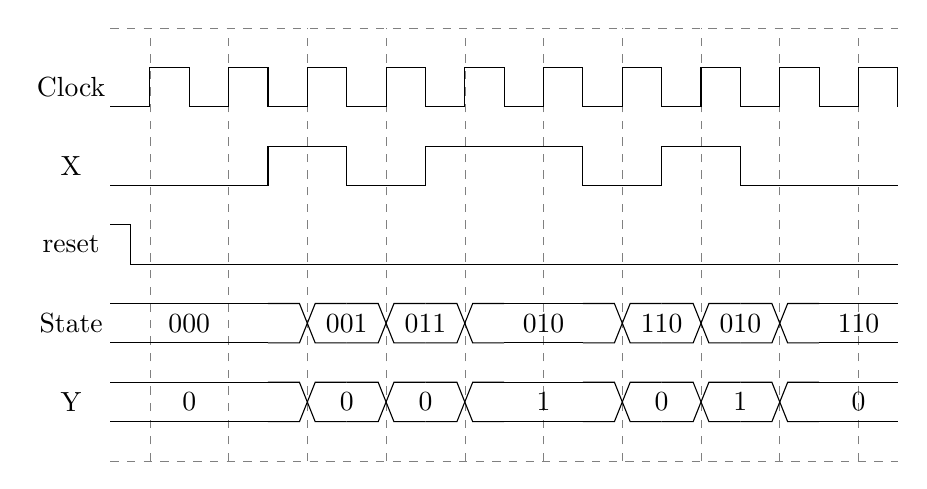
\begin{tikzpicture}
\draw [help lines,dashed] (-0.5,0) grid[xstep=1,ystep=5.5] (9.5,5.5);
\foreach \i in {0,...,9} {
	\draw (\i-0.5,4.5) -- (\i,4.5) -- (\i,5) -- (\i+0.5,5) -- (\i+0.5,4.5);
}
\draw plot[const plot] coordinates {(-0.5,3.5) (1.5,4) (2.5,3.5) (3.5,4) (5.5,3.5) (6.5,4) (7.5,3.5) (9.5,3.5)};
\draw plot[const plot] coordinates {(-0.5,3) (-0.25,2.5) (9.5,2.5)};
\foreach \j in {1,2} {
	\foreach \i in {2,3,4,6,7,8} {
		\draw (\i-0.5,\j) -- (\i-0.1,\j) -- (\i+0.1,\j-0.5) -- (\i+0.5,\j-0.5);
		\draw (\i-0.5,\j-0.5) -- (\i-0.1,\j-0.5) -- (\i+0.1,\j) -- (\i+0.5,\j);
	}
	\foreach \i in {0,1,5,9} {
		\draw (\i-0.5,\j) -- (\i+0.5,\j);
		\draw (\i-0.5,\j-0.5) -- (\i+0.5,\j-0.5);
	}
}
\draw (0.5,1.75) node {000} (2.5,1.75) node {001} (3.5,1.75) node {011} (5,1.75) node {010} (6.5,1.75) node {110} (7.5,1.75) node {010} (9,1.75) node {110};
\draw (0.5,0.75) node {0} (2.5,0.75) node {0} (3.5,0.75) node {0} (5,0.75) node {1} (6.5,0.75) node {0} (7.5,0.75) node {1} (9,0.75) node {0};
\draw (-1,4.75) node {Clock} (-1,3.75) node {X} (-1,2.75) node {reset} (-1,1.75) node {State} (-1,0.75) node {Y};
\end{tikzpicture}
\end{center}
\item
The state diagram is

\begin{center}
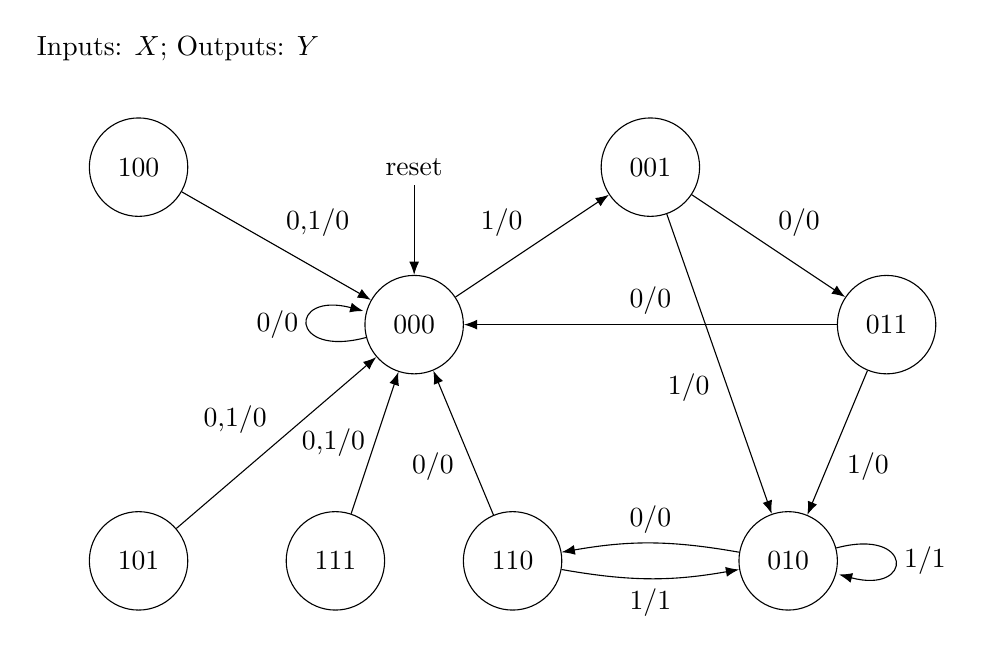
\begin{tikzpicture}[>/.tip={Latex}]
	\draw (-6,2) node (io) {Inputs: $X$; Outputs: $Y$};
	
	\draw (-3,-1.5) node (A) [draw,shape=circle,minimum size=1.25cm,text width=0.75cm,align=center] {000};
	\draw (0,0.5) node (B) [draw,shape=circle,minimum size=1.25cm,text width=0.75cm,align=center] {001};
	\draw (3,-1.5) node (C) [draw,shape=circle,minimum size=1.25cm,text width=0.75cm,align=center] {011};
	\draw (1.75,-4.5) node (D) [draw,shape=circle,minimum size=1.25cm,text width=0.75cm,align=center] {010};
	\draw (-1.75,-4.5) node (E) [draw,shape=circle,minimum size=1.25cm,text width=0.75cm,align=center] {110};
	
	\draw (-6.5,0.5) node (F) [draw,shape=circle,minimum size=1.25cm,text width=0.75cm,align=center] {100};
	\draw (-6.5,-4.5) node (G) [draw,shape=circle,minimum size=1.25cm,text width=0.75cm,align=center] {101};
	\draw (-4,-4.5) node (H) [draw,shape=circle,minimum size=1.25cm,text width=0.75cm,align=center] {111};

	\draw[->] (A) edge [loop left] node {0/0} ();
	\draw[->] (A) edge node [above left] {1/0} (B);
	\draw[->] (B) edge node [above right] {0/0} (C);
	\draw[->] (B) edge node [below left] {1/0} (D);
	\draw[->] (C) edge node [above] {0/0} (A);
	\draw[->] (C) edge node [below right] {1/0} (D);
	\draw[->] (D) edge [bend right=10] node [above] {0/0} (E);
	\draw[->] (D) edge [loop right] node {1/1} ();
	\draw[->] (E) edge node [below left] {0/0} (A);
	\draw[->] (E) edge [bend right=10] node [below] {1/1} (D);
	
	\draw[->] (F) edge node [above right] {0,1/0} (A);
	\draw[->] (G) edge node [above left] {0,1/0} (A);
	\draw[->] (H) edge node [left] {0,1/0} (A);
	
	\draw (-3,0.5) node (reset) {reset};
	\draw[->] (reset) edge (A);
\end{tikzpicture}
\end{center}

The truth table is 

\begin{center}
\begin{tabular}{cccc|cccc}
$s_{2}$ & $s_{1}$ & $s_{0}$ & $X$ & $n_{2}$ & $n_{1}$ & $n_{0}$ & $Y$ \\
\hline
0 & 0 & 0 & 0 & 0 & 0 & 0 & 0 \\
0 & 0 & 0 & 1 & 0 & 0 & 1 & 0 \\
0 & 0 & 1 & 0 & 0 & 1 & 1 & 0 \\
0 & 0 & 1 & 1 & 0 & 1 & 0 & 0 \\
0 & 1 & 0 & 0 & 1 & 1 & 0 & 0 \\
0 & 1 & 0 & 1 & 0 & 1 & 0 & 1 \\
0 & 1 & 1 & 0 & 0 & 0 & 0 & 0 \\
0 & 1 & 1 & 1 & 0 & 1 & 0 & 0 \\
1 & 0 & 0 & 0 & 0 & 0 & 0 & 0 \\
1 & 0 & 0 & 1 & 0 & 0 & 0 & 0 \\
1 & 0 & 1 & 0 & 0 & 0 & 0 & 0 \\
1 & 0 & 1 & 1 & 0 & 0 & 0 & 0 \\
1 & 1 & 0 & 0 & 0 & 0 & 0 & 0 \\
1 & 1 & 0 & 1 & 0 & 1 & 0 & 1 \\
1 & 1 & 1 & 0 & 0 & 0 & 0 & 0 \\
1 & 1 & 1 & 1 & 0 & 0 & 0 & 0 \\
\end{tabular}
\end{center}

The euqations are 

$$n_{2}=s_{2}'s_{1}s_{0}'X'$$
$$n_{1}=s_{2}'s_{1}'s_{0}+s_{2}'s_{0}X+s_{2}'s_{1}s_{0}'+s_{1}s_{0}'X$$
$$n_{0}=s_{2}'s_{1}'s_{0}'X+s_{2}'s_{1}'s_{0}X'$$
$$Y=s_{1}s_{0}'X$$


The schematics is 

\begin{center}
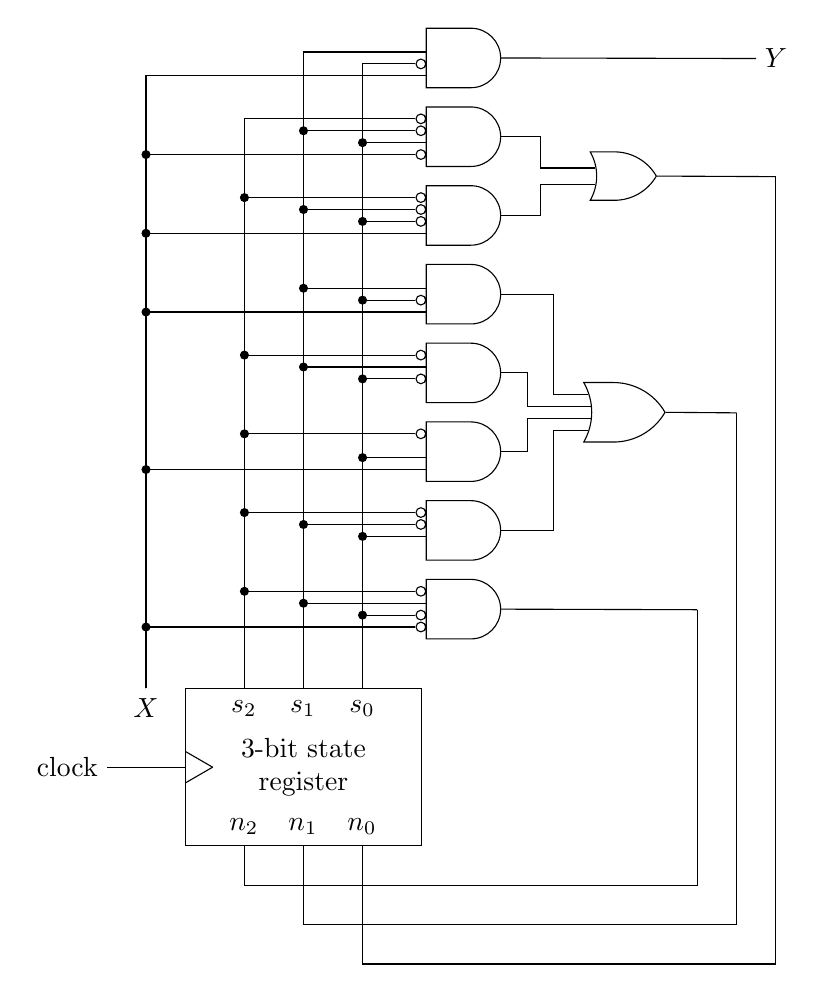
\begin{tikzpicture}[circuit logic US]
\draw (0,0) node (r) [shape=rectangle,draw,minimum height=2cm,minimum width=3cm,text width=2cm,align=center] {3-bit state register};
\draw (-3,0) node (clock) {clock};\draw (clock) -- (r.west);\draw (r) ++(left:11.54mm) -- ++($(left:3.46mm)+(down:2mm)$);
\draw (r) ++(left:11.54mm) -- ++($(left:3.46mm)+(up:2mm)$);
\draw (r.west) ++(up:7.5mm) ++(right:7.500000mm) node {$s_2$};
\draw (r.west) ++(down:7.5mm) ++(right:7.500000mm) node {$n_2$};
\draw (r.west) ++(up:7.5mm) ++(right:15.000000mm) node {$s_1$};
\draw (r.west) ++(down:7.5mm) ++(right:15.000000mm) node {$n_1$};
\draw (r.west) ++(up:7.5mm) ++(right:22.500000mm) node {$s_0$};
\draw (r.west) ++(down:7.5mm) ++(right:22.500000mm) node {$n_0$};
\draw (-2.000000,0.750000) node {$X$};
\draw (r.north) ++(up:1.000000cm) ++(right:2cm) node (and1) [and gate,inputs=inii] {};
\draw (-0.750000,1.000000) |- (and1.input 1) ;
\draw (0.000000,1.000000) |- (and1.input 2) ;
\draw (0.750000,1.000000) |- (and1.input 3) ;
\draw (-2.000000,1.000000) |- (and1.input 4) ;
\draw (and1.output) -- (5.000000,2.000000);
\draw (5.000000,2.000000) -- (5.000000,-1.500000) -| (-0.750000,-1);
\draw (r.north) ++(up:2.000000cm) ++(right:2cm) node (and2) [and gate,inputs=iinn] {};
\draw (-0.750000,1.000000) |- (and2.input 1) ;
\draw (0.000000,1.000000) |- (and2.input 2) ;
\draw (0.750000,1.000000) |- (and2.input 3) ;
\draw (and1.input 1) ;
\pgfgetlastxy{\x}{\y};
\filldraw (-0.750000,\y) circle [radius=0.5mm];
\draw (and1.input 2) ;
\pgfgetlastxy{\x}{\y};
\filldraw (0.000000,\y) circle [radius=0.5mm];
\draw (and1.input 3) ;
\pgfgetlastxy{\x}{\y};
\filldraw (0.750000,\y) circle [radius=0.5mm];
\draw (r.north) ++(up:3.000000cm) ++(right:2cm) node (and3) [and gate,inputs=innn] {};
\draw (-0.750000,1.000000) |- (and3.input 1) ;
\draw (0.750000,1.000000) |- (and3.input 3) ;
\draw (-2.000000,1.000000) |- (and3.input 4) ;
\draw (and2.input 1) ;
\pgfgetlastxy{\x}{\y};
\filldraw (-0.750000,\y) circle [radius=0.5mm];
\draw (and2.input 3) ;
\pgfgetlastxy{\x}{\y};
\filldraw (0.750000,\y) circle [radius=0.5mm];
\draw (and1.input 4) ;
\pgfgetlastxy{\x}{\y};
\filldraw (-2.000000,\y) circle [radius=0.5mm];
\draw (r.north) ++(up:4.000000cm) ++(right:2cm) node (and4) [and gate,inputs=inin] {};
\draw (-0.750000,1.000000) |- (and4.input 1) ;
\draw (0.000000,1.000000) |- (and4.input 2) ;
\draw (0.750000,1.000000) |- (and4.input 3) ;
\draw (and3.input 1) ;
\pgfgetlastxy{\x}{\y};
\filldraw (-0.750000,\y) circle [radius=0.5mm];
\draw (and2.input 2) ;
\pgfgetlastxy{\x}{\y};
\filldraw (0.000000,\y) circle [radius=0.5mm];
\draw (and3.input 3) ;
\pgfgetlastxy{\x}{\y};
\filldraw (0.750000,\y) circle [radius=0.5mm];
\draw (r.north) ++(up:5.000000cm) ++(right:2cm) node (and5) [and gate,inputs=nnin] {};
\draw (0.000000,1.000000) |- (and5.input 2) ;
\draw (0.750000,1.000000) |- (and5.input 3) ;
\draw (-2.000000,1.000000) |- (and5.input 4) ;
\draw (and4.input 2) ;
\pgfgetlastxy{\x}{\y};
\filldraw (0.000000,\y) circle [radius=0.5mm];
\draw (and4.input 3) ;
\pgfgetlastxy{\x}{\y};
\filldraw (0.750000,\y) circle [radius=0.5mm];
\draw (and3.input 4) ;
\pgfgetlastxy{\x}{\y};
\filldraw (-2.000000,\y) circle [radius=0.5mm];
\draw (r.north) ++(up:3.500000cm) ++(right:4cm) node (or2) [or gate,inputs=nnnn] {};
\draw (and2.output) -- ++(right:0.666667cm) |- (or2.input 4);
\draw (and3.output) -- ++(right:0.333333cm) |- (or2.input 3);
\draw (and4.output) -- ++(right:0.333333cm) |- (or2.input 2);
\draw (and5.output) -- ++(right:0.666667cm) |- (or2.input 1);
\draw (or2.output) -- (5.500000,4.500000);
\draw (5.500000,4.500000) -- (5.500000,-2.000000) -| (0.000000,-1);
\draw (r.north) ++(up:6.000000cm) ++(right:2cm) node (and6) [and gate,inputs=iiin] {};
\draw (-0.750000,1.000000) |- (and6.input 1) ;
\draw (0.000000,1.000000) |- (and6.input 2) ;
\draw (0.750000,1.000000) |- (and6.input 3) ;
\draw (-2.000000,1.000000) |- (and6.input 4) ;
\draw (and4.input 1) ;
\pgfgetlastxy{\x}{\y};
\filldraw (-0.750000,\y) circle [radius=0.5mm];
\draw (and5.input 2) ;
\pgfgetlastxy{\x}{\y};
\filldraw (0.000000,\y) circle [radius=0.5mm];
\draw (and5.input 3) ;
\pgfgetlastxy{\x}{\y};
\filldraw (0.750000,\y) circle [radius=0.5mm];
\draw (and5.input 4) ;
\pgfgetlastxy{\x}{\y};
\filldraw (-2.000000,\y) circle [radius=0.5mm];
\draw (r.north) ++(up:7.000000cm) ++(right:2cm) node (and7) [and gate,inputs=iini] {};
\draw (-0.750000,1.000000) |- (and7.input 1) ;
\draw (0.000000,1.000000) |- (and7.input 2) ;
\draw (0.750000,1.000000) |- (and7.input 3) ;
\draw (-2.000000,1.000000) |- (and7.input 4) ;
\draw (and6.input 1) ;
\pgfgetlastxy{\x}{\y};
\filldraw (-0.750000,\y) circle [radius=0.5mm];
\draw (and6.input 2) ;
\pgfgetlastxy{\x}{\y};
\filldraw (0.000000,\y) circle [radius=0.5mm];
\draw (and6.input 3) ;
\pgfgetlastxy{\x}{\y};
\filldraw (0.750000,\y) circle [radius=0.5mm];
\draw (and6.input 4) ;
\pgfgetlastxy{\x}{\y};
\filldraw (-2.000000,\y) circle [radius=0.5mm];
\draw (r.north) ++(up:6.500000cm) ++(right:4cm) node (or3) [or gate,inputs=nn] {};
\draw (and6.output) -- ++(right:0.500000cm) |- (or3.input 2);
\draw (and7.output) -- ++(right:0.500000cm) |- (or3.input 1);
\draw (or3.output) -- (6.000000,7.500000);
\draw (6.000000,7.500000) -- (6.000000,-2.500000) -| (0.750000,-1);
\draw (r.north) ++(up:8.000000cm) ++(right:2cm) node (and8) [and gate,inputs=nnin] {};
\draw (0.000000,1.000000) |- (and8.input 2) ;
\draw (0.750000,1.000000) |- (and8.input 3) ;
\draw (-2.000000,1.000000) |- (and8.input 4) ;
\draw (and7.input 2) ;
\pgfgetlastxy{\x}{\y};
\filldraw (0.000000,\y) circle [radius=0.5mm];
\draw (and7.input 3) ;
\pgfgetlastxy{\x}{\y};
\filldraw (0.750000,\y) circle [radius=0.5mm];
\draw (and7.input 4) ;
\pgfgetlastxy{\x}{\y};
\filldraw (-2.000000,\y) circle [radius=0.5mm];
\draw (and8.output) -- (5.750000,9.000000);
\draw (6,9.000000) node {$Y$};
\end{tikzpicture}
\end{center}

\end{enumerate}

\section{}

\newcommand{\drawcross}[2]{
	\draw (#1,#2) -- (#1+1,#2+1) (#1,#2+1) -- (#1+1,#2);
}
\newcommand{\drawtextt}[4]{
	\draw (#1+0.5,#2+0.75) node {(#3)};
	\draw (#1+0.5,#2+0.25) node {(#4)};
}
\newcommand{\drawtext}[3]{
	\draw (#1+0.5,#2+0.5) node {(#3)};
}

\begin{center}
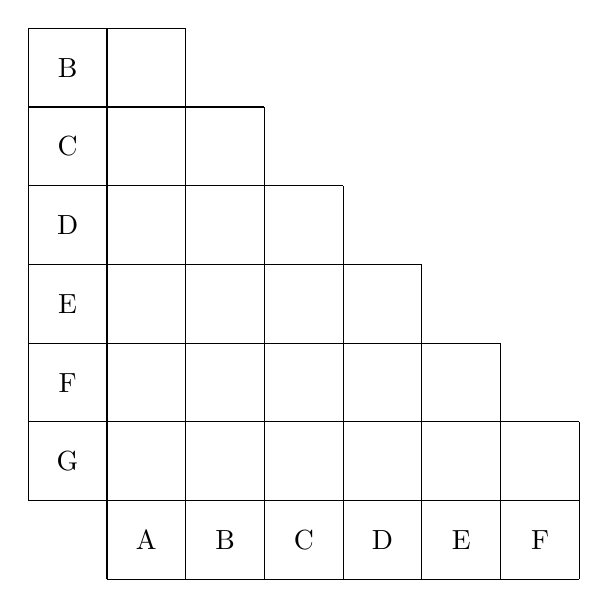
\begin{tikzpicture}
	\foreach \i in {1,...,6} {
		\draw (-1,\i) -- (7-\i, \i);
		\draw (\i,-1) -- (\i, 7-\i);
	}
	\draw (-1,0) -- (6,0) (0,-1) -- (0,6);
	\draw (0,-1) -- (6,-1) (-1,0) -- (-1,6);
	\foreach \i/\j in {1/G,2/F,3/E,4/D,5/C,6/B} {
		\draw (-0.5,\i-0.5) node {\j};
	}
	\foreach \i/\j in {1/A,2/B,3/C,4/D,5/E,6/F} {
		\draw (\i-0.5,-0.5) node {\j};
	}
	\drawcross{0}{5};
	\drawcross{0}{4};
	\drawcross{1}{0};
	\drawcross{1}{1};
	\drawcross{1}{2};
	\drawcross{1}{3};
	\drawcross{2}{0};
	\drawcross{2}{1};
	\drawcross{2}{2};
	\drawcross{2}{3};
	\drawtextt{0}{0}{C,F}{B,F};
	\drawtextt{0}{1}{F,F}{E,F};
	\drawtextt{0}{2}{G,F}{E,F};
	\drawtext {0}{3}{F,F};
	\drawtextt{1}{4}{E,E}{D,A};
	\drawtextt{3}{0}{C,F}{B,F};
	\drawtextt{3}{1}{F,F}{E,F};
	\drawtextt{3}{2}{G,F}{E,F};
	\drawtextt{4}{0}{C,G}{B,E};
	\drawtextt{4}{1}{F,G}{E,E};
	\drawtextt{5}{0}{C,F}{B,E};
	\drawcross{0}{0};
	\drawcross{3}{0};
	\drawcross{5}{0};
	\drawcross{4}{1};
	\drawcross{0}{2};
	\drawcross{3}{1};
	\drawcross{3}{2};
	\drawcross{0}{1};
	\drawcross{4}{0};
\end{tikzpicture}
\end{center}

So we can find that (A,D) and (B,C) are two pairs of equivalent state.

The optimized FSM diagram is

\begin{center}
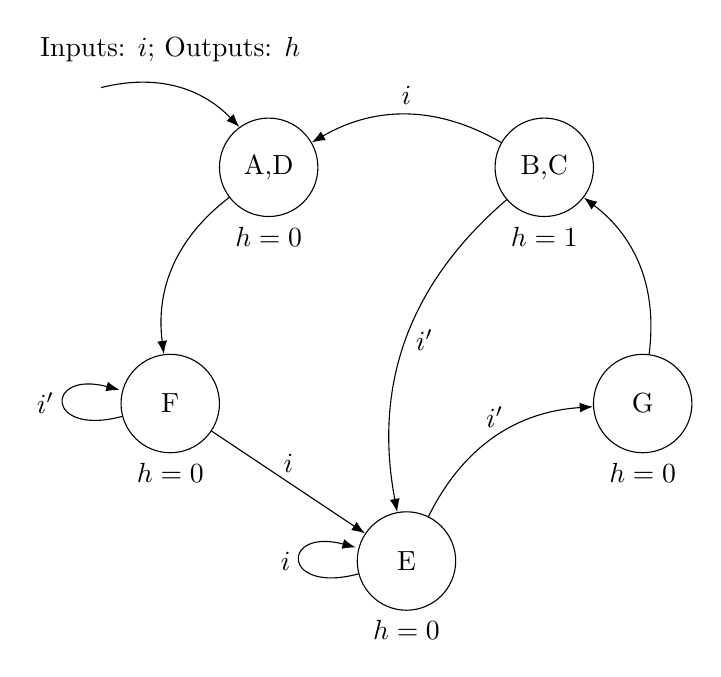
\begin{tikzpicture}[>/.tip={Latex}]
	\draw (-3,0.5) node (io) {Inputs: $i$; Outputs: $h$};
	
	\draw (-1.75,-1) node (A) [draw,shape=circle,minimum size=1.25cm] {A,D};
	\node [below] at (A.south) {$h=0$};
	\draw (1.75,-1) node (B) [draw,shape=circle,minimum size=1.25cm] {B,C};
	\node [below] at (B.south) {$h=1$};
	\draw (-3,-4) node (F) [draw,shape=circle,minimum size=1.25cm] {F};
	\node [below] at (F.south) {$h=0$};
	\draw (3,-4) node (G) [draw,shape=circle,minimum size=1.25cm] {G};
	\node [below] at (G.south) {$h=0$};
	\draw (0,-6) node (E) [draw,shape=circle,minimum size=1.25cm] {E};
	\node [below] at (E.south) {$h=0$};

	\draw[->] (A) edge [bend right=30] node {} (F);
	\draw[->] (B) edge [bend right=30] node [right] {$i'$} (E);
	\draw[->] (B) edge [bend right=30] node [above] {$i$} (A);
	\draw[->] (E) edge [bend left=30] node [above] {$i'$} (G);
	\draw[->] (E) edge [loop left] node {$i$} ();
	\draw[->] (F) edge [loop left] node {$i'$} ();
	\draw[->] (F) edge node [above] {$i$} (E);
	\draw[->] (G) edge [bend right=30] node {} (B);
	
	\draw (-4,0) node (init) {};
	\draw[->] (init) edge [bend left=30] (A);
\end{tikzpicture}
\end{center}

\section{}
Straightforward 2-bit binary encoding:

The truth table is 

\begin{center}
\begin{tabular}{cc|ccccc}
$s_{1}$ & $s_{0}$ & $n_{1}$ & $n_{0}$ & $W$ & $X$ & $Y$ \\
\hline
0 & 0 & 0 & 1 & 1 & 0 & 0 \\
0 & 1 & 1 & 0 & 0 & 1 & 0 \\
1 & 0 & 1 & 1 & 0 & 0 & 1 \\
1 & 1 & 0 & 0 & 0 & 0 & 0 \\
\end{tabular}
\end{center}

The euqations are 

$$n_{1}=s_{1}'s_{0}+s_{1}s_{0}'$$
$$n_{0}=s_{0}'$$
$$W=s_{1}'s_{0}'$$
$$X=s_{1}'s_{0}$$
$$Y=s_{1}s_{0}'$$




The logic size is 8, the delay is 1.\\

3-bit output encoding:

The truth table is 

\begin{center}
\begin{tabular}{ccc|cccccc}
$s_{2}$ & $s_{1}$ & $s_{0}$ & $n_{2}$ & $n_{1}$ & $n_{0}$ & $W$ & $X$ & $Y$ \\
\hline
0 & 0 & 0 & 1 & 0 & 0 & 0 & 0 & 0 \\
0 & 0 & 1 & 0 & 0 & 0 & 0 & 0 & 1 \\
0 & 1 & 0 & 0 & 0 & 1 & 0 & 1 & 0 \\
0 & 1 & 1 & X & X & X & X & X & X \\
1 & 0 & 0 & 0 & 1 & 0 & 1 & 0 & 0 \\
1 & 0 & 1 & X & X & X & X & X & X \\
1 & 1 & 0 & X & X & X & X & X & X \\
1 & 1 & 1 & X & X & X & X & X & X \\
\end{tabular}
\end{center}

The euqations are 

$$n_{2}=s_{2}'s_{1}'s_{0}'$$
$$n_{1}=s_{2}$$
$$n_{0}=s_{1}$$
$$W=s_{2}$$
$$X=s_{1}$$
$$Y=s_{0}$$




The logic size is 3, the delay is 1.\\

One-hot encoding:

The truth table is 

\begin{center}
\begin{tabular}{cccc|ccccccc}
$s_{3}$ & $s_{2}$ & $s_{1}$ & $s_{0}$ & $n_{3}$ & $n_{2}$ & $n_{1}$ & $n_{0}$ & $W$ & $X$ & $Y$ \\
\hline
0 & 0 & 0 & 0 & X & X & X & X & X & X & X \\
0 & 0 & 0 & 1 & 0 & 0 & 1 & 0 & 1 & 0 & 0 \\
0 & 0 & 1 & 0 & 0 & 1 & 0 & 0 & 0 & 1 & 0 \\
0 & 0 & 1 & 1 & X & X & X & X & X & X & X \\
0 & 1 & 0 & 0 & 1 & 0 & 0 & 0 & 0 & 0 & 1 \\
0 & 1 & 0 & 1 & X & X & X & X & X & X & X \\
0 & 1 & 1 & 0 & X & X & X & X & X & X & X \\
0 & 1 & 1 & 1 & X & X & X & X & X & X & X \\
1 & 0 & 0 & 0 & 0 & 0 & 0 & 1 & 0 & 0 & 0 \\
1 & 0 & 0 & 1 & X & X & X & X & X & X & X \\
1 & 0 & 1 & 0 & X & X & X & X & X & X & X \\
1 & 0 & 1 & 1 & X & X & X & X & X & X & X \\
1 & 1 & 0 & 0 & X & X & X & X & X & X & X \\
1 & 1 & 0 & 1 & X & X & X & X & X & X & X \\
1 & 1 & 1 & 0 & X & X & X & X & X & X & X \\
1 & 1 & 1 & 1 & X & X & X & X & X & X & X \\
\end{tabular}
\end{center}

The euqations are 

$$n_{3}=s_{2}$$
$$n_{2}=s_{1}$$
$$n_{1}=s_{0}$$
$$n_{0}=s_{3}$$
$$W=s_{0}$$
$$X=s_{1}$$
$$Y=s_{2}$$




The logic size is 0, the delay is 0.\\

\end{document}
